\documentclass[10pt,a4paper]{article}

% ===============================================================================
% PREAMBLE & PACKAGES
% ===============================================================================
\usepackage{fontspec}
\setmainfont{Latin Modern Roman}
\setmonofont{Latin Modern Mono}
\usepackage{unicode-math}
\setmathfont{Latin Modern Math}

\usepackage[margin=0.7in,top=0.9in,bottom=0.9in]{geometry}
\usepackage{xcolor}
\usepackage{tikz}
\usetikzlibrary{shapes.geometric, arrows.meta, positioning, calc, fit, decorations.pathreplacing}
\usepackage[most]{tcolorbox}
\usepackage{tabularx}
\usepackage{array}
\usepackage{enumitem}
\usepackage{amsmath}
\usepackage{fancyhdr}
\usepackage{microtype}
\usepackage[colorlinks=true,linkcolor=myteal,citecolor=mypurple,urlcolor=myblue]{hyperref}

\hyphenpenalty=10000
\exhyphenpenalty=10000
\sloppy

% ===============================================================================
% COLOR PALETTE (Strict adherence to spec)
% ===============================================================================
\definecolor{myred}{RGB}{196,30,58}       % section headings
\definecolor{mydark}{RGB}{30,30,50}       % body text
\definecolor{mygreen}{RGB}{14,120,80}     % definition boxes
\definecolor{myteal}{RGB}{0,130,140}      % formula boxes, diagrams, subsection headings
\definecolor{myamber}{RGB}{180,100,0}     % example boxes
\definecolor{mypurple}{RGB}{100,30,160}   % exam/viva boxes
\definecolor{myblue}{RGB}{25,90,170}      % hyperlinks/diagrams
\definecolor{mygray}{RGB}{246,247,249}    % tikzbox background
\definecolor{mgframe}{RGB}{180,185,200}   % tikzbox border
\definecolor{watermark}{RGB}{145,150,170} % footer watermark

\definecolor{hdrred}{RGB}{250,232,235}
\definecolor{hdrgreen}{RGB}{220,244,233}
\definecolor{hdrteal}{RGB}{220,242,244}
\definecolor{hdramber}{RGB}{253,242,215}
\definecolor{hdrpurple}{RGB}{238,228,255}
\definecolor{hdrblue}{RGB}{235,242,250}

% ===============================================================================
% TCOLORBOX STYLES
% ===============================================================================
\tcbset{
  tikzbox/.style={colback=mygray, colframe=mgframe, boxrule=0.6pt, arc=4pt,
    left=8pt, right=8pt, top=6pt, bottom=6pt,
    colbacktitle=mgframe, coltitle=mydark, fonttitle=\small\bfseries},
  defbox/.style={colback=hdrgreen, colframe=mygreen, boxrule=0.8pt, arc=4pt,
    left=9pt, right=9pt, top=6pt, bottom=6pt,
    colbacktitle=mygreen, coltitle=white, fonttitle=\small\bfseries},
  formulabox/.style={colback=hdrteal, colframe=myteal, boxrule=0.8pt, arc=4pt,
    left=9pt, right=9pt, top=7pt, bottom=7pt,
    colbacktitle=myteal, coltitle=white, fonttitle=\small\bfseries},
  examplebox/.style={colback=hdramber, colframe=myamber, boxrule=0.8pt, arc=4pt,
    left=9pt, right=9pt, top=6pt, bottom=6pt,
    colbacktitle=myamber, coltitle=white, fonttitle=\small\bfseries},
  masonbox/.style={colback=hdrpurple, colframe=mypurple, boxrule=0.8pt, arc=4pt,
    left=9pt, right=9pt, top=6pt, bottom=6pt,
    colbacktitle=mypurple, coltitle=white, fonttitle=\small\bfseries},
  exambox/.style={colback=hdrpurple, colframe=mypurple, boxrule=1pt, arc=5pt,
    left=10pt, right=10pt, top=8pt, bottom=8pt,
    colbacktitle=mypurple, coltitle=white, fonttitle=\bfseries,
    title after break={\textbf{Frequently Asked / Viva Questions (contd.)}}}
}
\tcbset{breakable}

% ===============================================================================
% TIKZ STYLES
% ===============================================================================
\tikzset{
  block/.style={rectangle, draw=myteal, fill=hdrteal, text width=2.4cm, align=center, minimum height=0.95cm, font=\small, rounded corners=3pt, line width=0.7pt},
  arrow/.style={-Stealth, thick, color=mydark},
  line/.style={thick, color=mydark}
}

% ===============================================================================
% MACROS & COMMANDS
% ===============================================================================
\newcommand{\Q}[1]{\textbf{#1}\par\vspace{2pt}}
\newcolumntype{Y}{>{\raggedright\arraybackslash}X}
\newcolumntype{C}{>{\centering\arraybackslash}X}

% Header & Footer
\pagestyle{fancy}
\fancyhf{}
\fancyhead[L]{\small\color{mydark}\textbf{OE-EC804B} --- Microwave Integrated Circuits}
\fancyhead[R]{\small\color{myteal}\textbf{Module 3 Notes}}
\fancyfoot[C]{\small\color{mydark}\thepage}
\fancyfoot[R]{\small\color{watermark}\copyright\ Biraj Sarkar}
\renewcommand{\headrulewidth}{0.6pt}

\hypersetup{pdftitle={OE-EC804B Module 3 Exam Notes}}

\begin{document}

% ===============================================================================
% TITLE BLOCK
% ===============================================================================
\begin{center}
  {\LARGE\bfseries\color{myred} OE-EC804B --- Microwave Integrated Circuits}\\[5pt]
  {\normalsize\color{mydark} Semester VIII \quad$\bullet$\quad 3L:0T:0P \quad$\bullet$\quad 3 Credits}\\[3pt]
  {\normalsize\color{myteal}\textbf{Module 3 Exam Notes: Planar Lines-II (Slotline, Finlines \& CPW)}}\\[3pt]
  {\small\color{mydark} CGEC \;$|$\; B.Tech ECE (2023--27) \;$|$\; \textit{Biraj Sarkar}}
\end{center}
\vspace{2pt}
\noindent{\color{myred}\rule{\linewidth}{1.5pt}}
\vspace{2pt}

\hypersetup{linkcolor=mydark}
\tableofcontents
\hypersetup{linkcolor=myteal}
\newpage

% ===============================================================================
% 1. SLOT LINE ANALYSIS AND FIELD DISTRIBUTION
% ===============================================================================
\section{Slot Line Analysis and Field Distribution}

A \textbf{Slotline} consists of a narrow slot of width $W$ etched in a conductive metal plane coated on one side of a dielectric substrate ($\varepsilon_r$ of thickness $h$), leaving the reverse side unmetallized.

\begin{tcolorbox}[defbox, title={Slotline Structure \& Propagation Mode}]
  Slotline is a non-TEM planar transmission line supporting a \textbf{TE-like mode}. Electric field lines extend horizontally across the slot gap ($E_y$), while magnetic field lines form closed loops in the longitudinal plane ($H_z \ne 0, H_x \ne 0$). Because $H_z \ne 0$, slotline exhibits elliptical magnetic field polarization, making it ideally suited for integrating non-reciprocal ferrite components (such as isolators and circulators).
\end{tcolorbox}

\subsection{Transverse Resonance Method (TRM) Analysis}
Because slotline fields are non-TEM, electro-static Laplace equations fail to predict dispersion. The \textbf{Transverse Resonance Method (TRM)} models the transverse cross-section as an equivalent transmission line resonant system in the transverse $y$-direction.

\begin{tcolorbox}[formulabox, title={Transverse Resonance Condition}]
  Consider a transverse cut plane at $y = 0$ across the slot interface. At resonance, the sum of input admittances looking into the upper air region ($\vec{Y}_{up}$) and lower substrate region ($\overleftarrow{Y}_{down}$) must sum to zero:
  \begin{equation}
    \vec{Y}_{up}(y=0) + \overleftarrow{Y}_{down}(y=0) = 0
  \end{equation}
  Enforcing $\text{Im}\{Y_{total}(\beta)\} = 0$ yields the guided wavenumber $\beta = 2\pi/\lambda_g$. Characteristic impedance $Z_0$ is evaluated from root-mean-square slot voltage $V$:
  \begin{equation}
    Z_0 = \frac{V^2}{2 P_{avg}} \quad \text{where } V = \int_{-W/2}^{W/2} E_y(x) dx
  \end{equation}
\end{tcolorbox}

\subsection{Exhaustive Comparison: Slotline vs. Microstrip Line}

\par\vspace{6pt}\noindent
\begingroup
\renewcommand{\arraystretch}{1.4}%
\begin{tabularx}{\linewidth}{|>{\raggedright\arraybackslash\bfseries}p{3.2cm}|Y|Y|}
\hline
\textbf{Parameter} & \textbf{Microstrip Line} & \textbf{Slotline} \\
\hline
Dominant Mode & Quasi-TEM mode ($E_z, H_z \approx 0$) & Non-TEM / TE-like mode ($H_z \ne 0$) \\
\hline
Field Distribution & Electric fields confined under central strip & Electric fields concentrated across slot gap \\
\hline
Shunt Mounting & Requires via holes drilled through substrate to ground & Direct surface mounting of active dies across slot without via holes \\
\hline
Series Mounting & Easy in-line series trace breaking & Difficult series connection \\
\hline
Impedance Range & $20\text{ }\Omega$ to $120\text{ }\Omega$ (Low impedance lines) & $50\text{ }\Omega$ to $300\text{ }\Omega$ (High impedance lines) \\
\hline
Magnetic Polarization & Linear transverse magnetic fields & Elliptically polarized $H$-field (Ideal for Ferrite devices) \\
\hline
Radiation Loss & Moderate at microwave frequencies & Slightly higher due to wide open top slot \\
\hline
\end{tabularx}
\endgroup

% ===============================================================================
% 2. COPLANAR WAVEGUIDE (CPW) AND FIN LINES
% ===============================================================================
\section{Coplanar Waveguide (CPW) and Fin Lines}

\subsection{Coplanar Waveguide (CPW)}
A \textbf{Coplanar Waveguide (CPW)} consists of a central signal conductor of width $W$ flanked by two semi-infinite ground planes on the \textbf{same top surface} of a dielectric substrate ($\varepsilon_r$), separated by narrow gaps $S$.

\begin{tcolorbox}[masonbox, title={Coplanar Waveguide (CPW) Advantages}]
  CPW supports a Quasi-TEM mode. Because both signal conductor and ground planes reside on the same face, both series and shunt components can be mounted \textbf{without drilling via holes}, significantly reducing MMIC manufacturing cost and parasitic via-inductance ($L_{via} \approx 0.1\text{ nH}$).
\end{tcolorbox}

\subsection{CPW Conformal Mapping \& Impedance Formulas}
Using conformal mapping, CPW effective dielectric constant $\varepsilon_{eff,CPW}$ and characteristic impedance $Z_{0,CPW}$ are derived in terms of complete elliptic integrals of the first kind $K(k)$:

\begin{tcolorbox}[formulabox, title={CPW Closed-Form Impedance Expressions}]
  \begin{equation}
    \varepsilon_{eff,CPW} = \frac{\varepsilon_r + 1}{2} \quad ; \quad Z_{0,CPW} = \frac{30\pi}{\sqrt{\varepsilon_{eff,CPW}}} \frac{K'(k)}{K(k)}
  \end{equation}
  where modulus $k = \frac{W}{W + 2S}$ and $K'(k) = K(k')$ with $k' = \sqrt{1 - k^2}$.
\end{tcolorbox}

\subsection{Fin Lines ($E$-Plane Waveguide Printed Lines)}
A \textbf{Finline} consists of a slotline printed on a thin dielectric substrate mounted along the central longitudinal $E$-plane of a rectangular metallic waveguide housing.

\begin{enumerate}[leftmargin=*, itemsep=4pt]
  \item \textbf{Unilateral Finline:} Slot printed on one face of the substrate only.
  \item \textbf{Bilateral Finline:} Identical slots printed symmetrically on both substrate faces.
  \item \textbf{Insulated Finline:} Substrate insulated from metallic waveguide top/bottom walls.
\end{enumerate}

\begin{tcolorbox}[tikzbox, title={Cross-Sections of Slotline, CPW, and Unilateral Finline}]
\centering
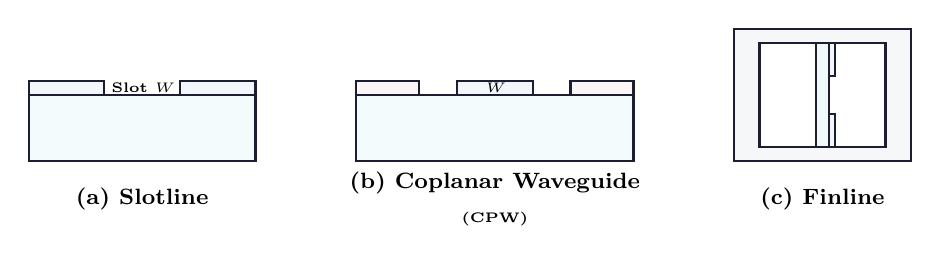
\begin{tikzpicture}[x=1.6cm, y=1.2cm]
  % Slotline
  \draw[line, fill=hdrteal!30] (0,0) rectangle (1.8,0.7);
  \draw[line, fill=hdrblue!60] (0,0.7) rectangle (0.6,0.85); % Left metal
  \draw[line, fill=hdrblue!60] (1.2,0.7) rectangle (1.8,0.85); % Right metal
  \node at (0.9,0.775) {\tiny\textbf{Slot $W$}};
  \node[align=center] at (0.9,-0.4) {\footnotesize\textbf{(a) Slotline}};
  
  % CPW
  \draw[line, fill=hdrteal!30] (2.6,0) rectangle (4.8,0.7);
  \draw[line, fill=hdrred!40] (2.6,0.7) rectangle (3.1,0.85); % Ground 1
  \draw[line, fill=hdrblue!60] (3.4,0.7) rectangle (4.0,0.85); % Center Strip
  \draw[line, fill=hdrred!40] (4.3,0.7) rectangle (4.8,0.85); % Ground 2
  \node at (3.7,0.775) {\tiny\textbf{$W$}};
  \node[align=center] at (3.7,-0.4) {\footnotesize\textbf{(b) Coplanar Waveguide}\\\tiny\textbf{(CPW)}};
  
  % Finline
  \draw[line, fill=mygray] (5.6,0) rectangle (7.0,1.4); % Waveguide box
  \draw[line, fill=white] (5.8,0.15) rectangle (6.8,1.25); % Inner cavity
  \draw[line, fill=hdrteal!40] (6.25,0.15) rectangle (6.35,1.25); % E-plane Substrate
  \draw[line, fill=hdrblue!60] (6.35,0.15) rectangle (6.4,0.5); % Bottom Fin
  \draw[line, fill=hdrblue!60] (6.35,0.9) rectangle (6.4,1.25); % Top Fin
  \node[align=center] at (6.3,-0.4) {\footnotesize\textbf{(c) Finline}};
\end{tikzpicture}
\end{tcolorbox}

\begin{tcolorbox}[examplebox, title={Worked Numerical: Coplanar Waveguide Impedance Calculation}]
  \textbf{Problem:} A Coplanar Waveguide (CPW) is fabricated on a GaAs substrate ($\varepsilon_r = 12.9$). Calculate:
  \begin{enumerate}[label=(\alph*), noitemsep]
    \item The effective dielectric constant $\varepsilon_{eff,CPW}$.
    \item The characteristic impedance $Z_0$ if ratio $K'(k)/K(k) = 1.0$.
  \end{enumerate}
  \tcblower
  \textbf{Solution:}
  \begin{enumerate}[label=(\alph*), itemsep=4pt]
    \item Effective dielectric constant for symmetrical CPW:
      \begin{equation}
        \varepsilon_{eff,CPW} = \frac{\varepsilon_r + 1}{2} = \frac{12.9 + 1}{2} = 6.95
      \end{equation}
    \item Characteristic impedance calculation:
      \begin{equation}
        Z_{0,CPW} = \frac{30\pi}{\sqrt{6.95}} \times (1.0) = \frac{94.2477}{2.63628} = 35.75\text{ }\Omega
      \end{equation}
  \end{enumerate}
\end{tcolorbox}

% ===============================================================================
% QUICK REVISION PAGE
% ===============================================================================
\newpage
\begin{center}
  {\large\bfseries\color{myred} Quick Revision --- Module 3}\\[3pt]
  {\small\color{mydark} Planar Lines-II (Slotline, Finlines \& CPW) $|$ OE-EC804B}
\end{center}
\noindent{\color{myred}\rule{\linewidth}{1.2pt}}
\vspace{4pt}

\begin{tcolorbox}[formulabox, title={\textbf{Key Concepts and Metrics at a Glance}}]
\renewcommand{\arraystretch}{1.35}
\begin{tabularx}{\linewidth}{>{\raggedright\arraybackslash\bfseries}p{4.5cm} X}
Slotline Mode & Non-TEM / TE-like mode with longitudinal magnetic field $H_z \ne 0$. \\[4pt]
Transverse Resonance Method & Evaluates slotline \& finline parameters via admittance resonance $\sum Y_{transverse} = 0$. \\[4pt]
CPW Effective Dielectric & $\varepsilon_{eff,CPW} = \frac{\varepsilon_r+1}{2}$ \quad (Equal electric energy split in air and substrate). \\[4pt]
CPW Impedance & $Z_{0,CPW} = \frac{30\pi}{\sqrt{\varepsilon_{eff}}} \frac{K'(k)}{K(k)}$ \quad (Using complete elliptic integrals). \\[4pt]
Via-Hole Elimination & CPW and Slotline allow direct surface shunt mounting of active devices without via holes. \\
\end{tabularx}
\end{tcolorbox}

\begin{tcolorbox}[defbox, title={\textbf{One-Line Definitions}}]
  \begin{itemize}[leftmargin=*, noitemsep]
    \item \textbf{Slotline:} A planar line formed by a narrow slot in a conductive ground plane on a dielectric substrate.
    \item \textbf{Coplanar Waveguide (CPW):} A planar line with center conductor and dual ground planes on the same surface.
    \item \textbf{Finline:} An $E$-plane slotline enclosed inside a rectangular waveguide wall.
    \item \textbf{Transverse Resonance Method (TRM):} Analytical field method enforcing zero net input admittance across transverse cut planes.
  \end{itemize}
\end{tcolorbox}

\begin{tcolorbox}[exambox, title={\textbf{Frequently Asked / Viva Questions}}]
  \begin{enumerate}[topsep=0pt, label=\textbf{Q\arabic*.}, itemsep=5pt]
    \item \Q{What is the dominant propagation mode in a slotline?}
    Slotline supports a non-TEM TE-like mode with a transverse electric field $E_y$ and longitudinal magnetic field $H_z$.

    \item \Q{Compare Slotline and Microstrip line.}
    Microstrip uses a Quasi-TEM mode with $20\text{ }\Omega$--$120\text{ }\Omega$ impedance and requires via holes for shunt mounting. Slotline uses a TE-like mode with $50\text{ }\Omega$--$300\text{ }\Omega$ impedance and allows direct surface shunt mounting.

    \item \Q{Why does Coplanar Waveguide (CPW) eliminate the need for via holes?}
    Because both signal conductor and ground planes reside on the top surface of the substrate, allowing active devices to be connected directly in shunt.

    \item \Q{Explain the Transverse Resonance Method (TRM).}
    TRM models the cross-section of a non-TEM transmission line as a transverse resonant line, finding $\beta$ by setting total transverse input admittance $\sum Y(y) = 0$.

    \item \Q{What is a Finline? Name its three main structural variations.}
    A Finline is an $E$-plane slotline enclosed inside a metallic rectangular waveguide. Variations: Unilateral, Bilateral, and Insulated Finlines.

    \item \Q{Why is slotline suitable for mounting non-reciprocal ferrite isolators?}
    Because the slotline magnetic field exhibits circular/elliptical polarization in the substrate region, ideal for ferrite interaction.

    \item \Q{How does the characteristic impedance of a CPW depend on gap width $S$?}
    Increasing gap width $S$ decreases total line capacitance, thereby increasing characteristic impedance $Z_0$.

    \item \Q{What is an air-bridge in CPW circuits?}
    A raised metal wire bridge connecting the dual ground planes of CPW to suppress unwanted odd-mode (slotline mode) propagation.

    \item \Q{What are the advantages of Finlines at millimeter-wave frequencies ($>30\text{ GHz}$)?}
    Combines the low loss and high power handling of rectangular waveguides with the planar circuit integration of slotlines.

    \item \Q{How does conductor loss $\alpha_c$ in Finlines vary with slot width $W$?}
    Conductor loss increases inversely with slot width ($1/W$) due to high current density concentration at fin edges.
  \end{enumerate}
\end{tcolorbox}

\end{document}
